\subsection{Datenverarbeitungskomponente}\label{sec:Datenverarbeitungskomponente}
Gem�� der Abbildung \ref{wissenserwerbskomponente} stellt die Datenverarbeitungskomponente ein Bindeglied zwischen der Wissensbasis (hier Git-Repository) und den Wissenserfassungsverfahren (z.B. Wissenstr�gerschnittstelle) dar. Auf Implementierung bezogen handelt es sich um ein Programm, das f�r eine kleine Aufgabe zust�ndig ist. Martin Flowler bezeichnet das als Mircoservice\footnote{https://www.martinfowler.com/articles/microservices.html}. Im Fall von \textit{PaaSfinder} wird dieser Microservice als \glqq{}Worker\grqq{} bezeichnet. Schematisch wird der Worker in Abbildung \ref{fig:worker} dargestellt.
\begin{figure}[H] 
	\centering
	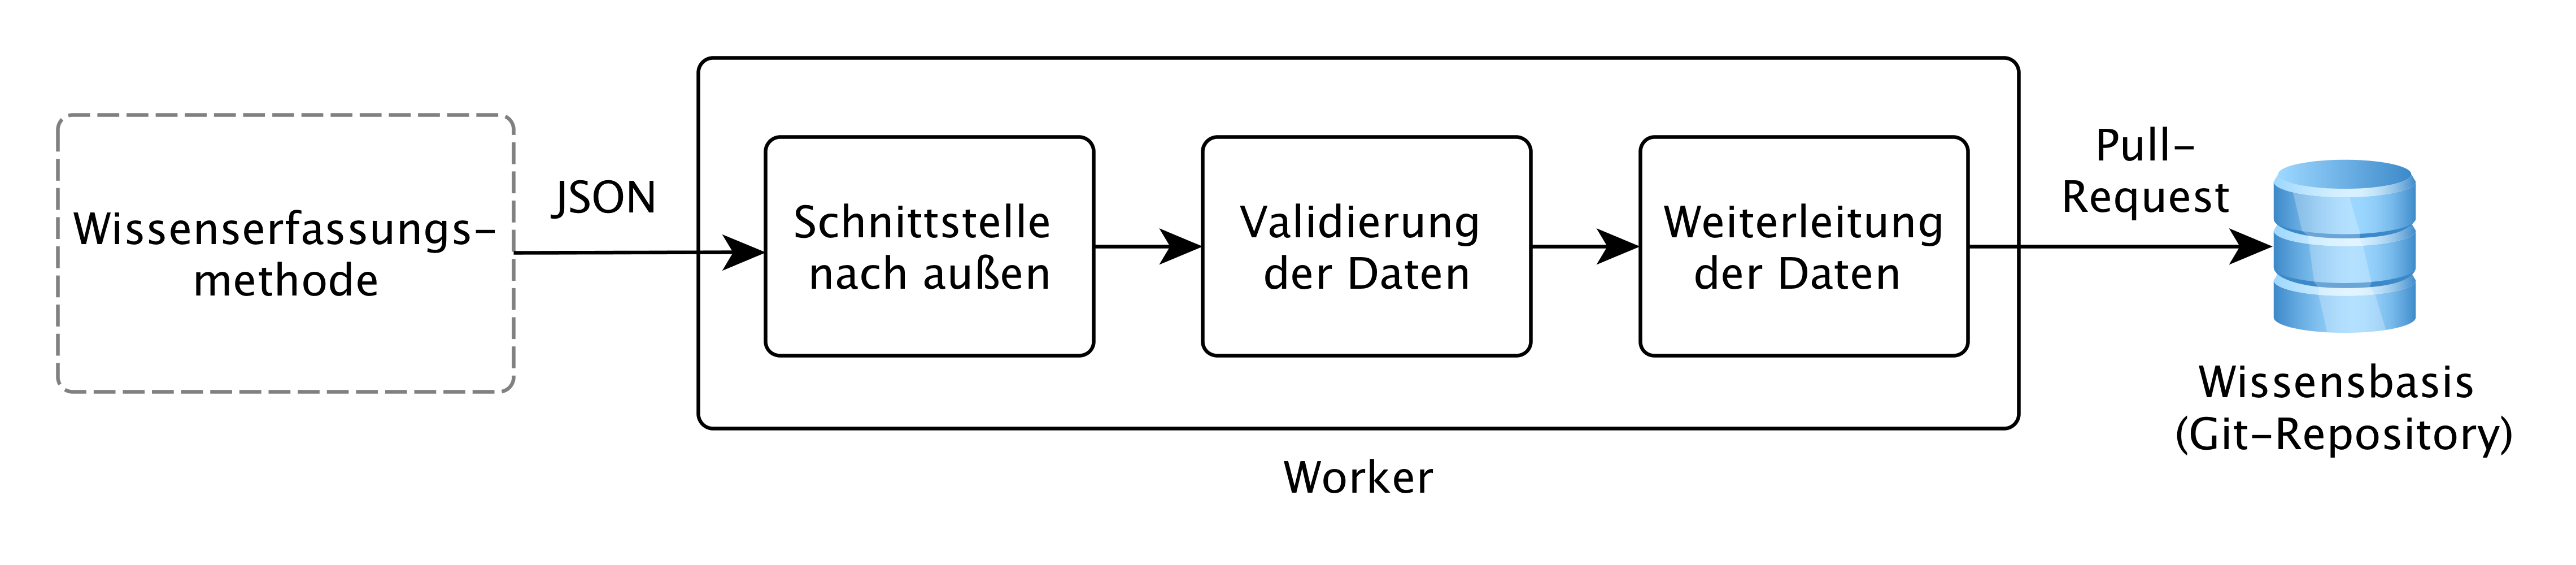
\includegraphics[width=1.0\textwidth]{images/worker.png}
	\caption{Der Aufgabenbereich vom Worker}
	\label{fig:worker}
\end{figure}
Der Aufgabenbereich vom Worker ist einfach. Zun�chst sollen die Daten durch eine Schnittstelle empfangen werden.  Dabei wird der Ausschlusskriterium angewandt, dass nur die Daten in JSON Format akzeptiert werden. Sobald die Daten vorliegen, werden sie im n�chste Schritt entsprechend f�r das Senden vorbereitet und an die Wissensbasis weitergegeben. In diesem Fall handelt es sich um die Erstellung eines Pull-Requests, der anschlie�emd an die Git-Repository gesendet wird.\\
Wie bereits angedeutet wurde, folgt die Implementierung des Workers dem REST-Architekturstil. \ac{REST} und dazugeh�rige Grundprinzipien nach \cite{tilkov2015} erl�utern.